\subsubsection{Compilation}

The compilation of a CUDA file follows a structured process that involves both the CPU and GPU components.
\begin{enumerate}
   \item \important{\texttt{.cu File}}. The source file containing CUDA kernels and the rest of the application code is usually saved with a \texttt{.cu} extension.

   \item \important{CUDA Kernels}. The CUDA-specific code within the \texttt{.cu} file is processed by the NVIDIA CUDA Compiler (NVCC). This includes all the functions intended to run on the GPU.

   \setcounter{enumi}{1}

   \item \important{Rest of the Application}. The non-CUDA parts of the code, intended to run on the CPU, are processed by the host CPU compiler.

   \item \important{NVCC Compiler}. NVCC compiles the CUDA kernels into CUDA object files, which are specific to the GPU.

   \setcounter{enumi}{2}

   \item \important{CPU Compiler}. The CPU compiler processes the remaining application code into CPU object files, which are specific to the CPU.

   \item \important{Linker}. The linker combines the CUDA object files and CPU object files into a single executable that can run on both the CPU and GPU.
\end{enumerate}
An example of a compilation is the command:
\begin{lstlisting}
nvcc -arch=sm_70 -o hello-gpu 01-hello/01-hello-gpu.cu -run
\end{lstlisting}
That demonstrates how to compile and execute a CUDA file using NVCC. The \texttt{-arch=sm\_70} flag specifies the architecture of the GPU, in this case, the Volta architecture (\texttt{sm\_70}).

\highspace
Useful Compilation Flags for NVCC:
\begin{table}[!htp]
   \centering
   \begin{tabular}{@{} l p{20em} @{}}
      \toprule
      \textbf{Flags} & \textbf{Description} \\
      \midrule
      \texttt{-x}          & Treat all input files as \texttt{.cu} files. \\
      \texttt{-Xcompiler}  & Pass a host compiler flag that is not supported by NVCC. \\
      \texttt{-g}          & Include host debugging symbols. \\
      \texttt{-G}          & Include device debugging symbols. \\
      \texttt{-lineinfo}   & Include line information with symbols. \\
      \bottomrule
   \end{tabular}
   \caption{Some compilation flags.}
\end{table}


\newpage

\begin{figure}[!htp]
   \centering
   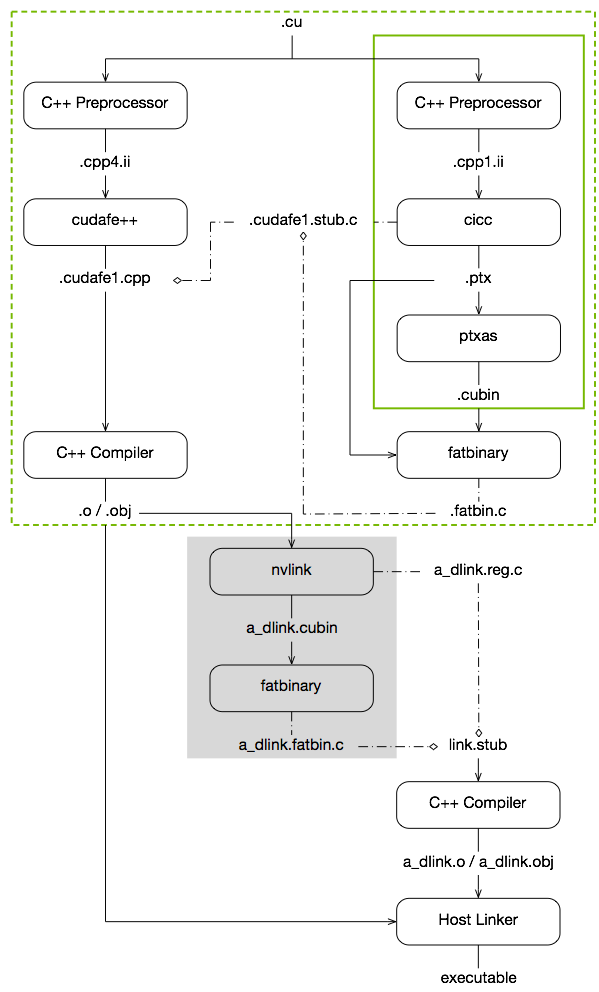
\includegraphics[width=.7\textwidth]{img/cuda-compilation-from-cu-to-executable-1.png}
   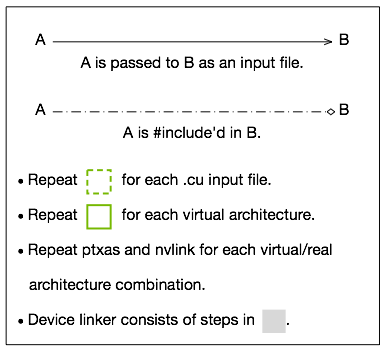
\includegraphics[width=.5\textwidth]{img/cuda-compilation-from-cu-to-executable-2.png}
   \caption{CUDA Compilation Trajectory, source: \href{https://docs.nvidia.com/cuda/cuda-compiler-driver-nvcc/index.html}{NVIDIA CUDA Compiler Driver NVCC}}
\end{figure}
